\documentclass{article}
\usepackage{graphicx}
\usepackage[margin=1.5cm]{geometry}
\usepackage{amsmath}

\begin{document}
\twocolumn

\title{Wednesday Reading Assessment: Unit 4, Power and Conservation of Energy}
\author{Prof. Jordan C. Hanson}

\maketitle

\section{Memory Bank}

\begin{itemize}
\item $W = \vec{F} \cdot \Delta \vec{x}$ ... Definition of work, Joules.
\item $P = dW/dt$ ... Definition of power, Watts.
\item $U = mg\Delta y$ ... Gravitational potential energy.
\item \textbf{Conservative force:}
\begin{equation}
\vec{F} = -\nabla U(x,y,z) = -\frac{\partial U}{\partial x}\hat{i}-\frac{\partial U}{\partial y}\hat{j}-\frac{\partial U}{\partial z}\hat{k}
\end{equation}
\item \textbf{Conservative force:}
\begin{equation}
\nabla \times \vec{F} = 0
\end{equation}
\end{itemize}

\begin{figure}
\centering
\includegraphics[width=0.2\textwidth]{pullup.png}
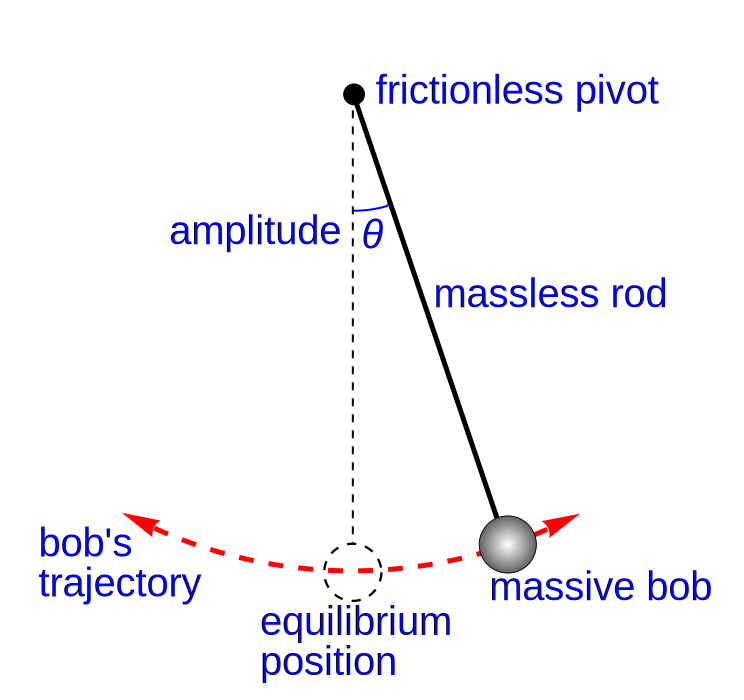
\includegraphics[width=0.2\textwidth]{pend.png}
\caption{\label{fig:work} (Left) An army trainee does pullups at a certain rate. (Right) A simple pendulum.}
\end{figure}

\section{Work and Power}

\begin{enumerate}
\item An 80-kg army trainee does 10 pull-ups in 10 seconds.  Assume the trainee raises his center of mass by $\Delta t = 0.6$ meters.  How much average power do the trainee’s muscles supply moving his body? \\ \vspace{2cm}
\item The unit of \textit{horsepower} is sometimes used to describe engines.  One horsepower is equal to 746 Watts.  (a) How many Watts can a 200 horsepower engine produce? (b) Another engine provides $3\times 10^6$ J of work in 1 hour.  How many horsepower does it have? \\ \vspace{2cm}
\end{enumerate}

\section{Conservation of Energy}

\begin{enumerate}
\item A particle of mass m is hung from the ceiling by a massless string of length 1.0 m, as shown in Figure \ref{fig:work}. The particle is released from rest, when the angle between the string and the downward vertical direction is 30 degrees.  What is its speed when it reaches the lowest point of its arc? \\ \vspace{3cm}
\item The \textit{partial derivative} $\partial U/\partial x$ is like taking the derivative with respect to one variable while holding the others constant. (a) Suppose $U(y) = mgy$.  What is $-\nabla U$? (b) Suppose $U(x,y) = \frac{1}{2}k(x^2+y^2)$.  What is $-\nabla U$? \\ \vspace{3cm}
\item A \textit{conservative force} obeys the following rule:
\begin{equation}
\nabla \times \vec{F} = 0
\end{equation}
This is called the \textit{curl} of the force.  A consequence of the rule is that
\begin{equation}
\frac{dF_x}{dy} = \frac{dF_y}{dx}
\end{equation}
Suppose $\vec{F} = -k(x\hat{i} + y\hat{j})$.  Does this force conserve energy?  What type of system is described by such a force?
\end{enumerate}

\end{document}